\chapter{Introduction}
\label{chap:introduction}

\section{Problem Introduction}
通过本课程的学习,我们知道通过若干张图像,我们可以同时获得图像中所拍摄场景的三维信息,并得到图像拍摄时的6个自由度的姿态和位置。

本课程大作业问题内容是使用自己的手机或相机,对同一个场景,分别在三个角度拍摄三张图像,最终获得三张图像拍摄时的姿态和位置,以及图像中特征点的三维坐标信息,并评估和验证所实现算法的正确性和精度性能。在本次实验中,我使用iphone手机拍摄的照片为交大“庙门”。三张图片如图所示:

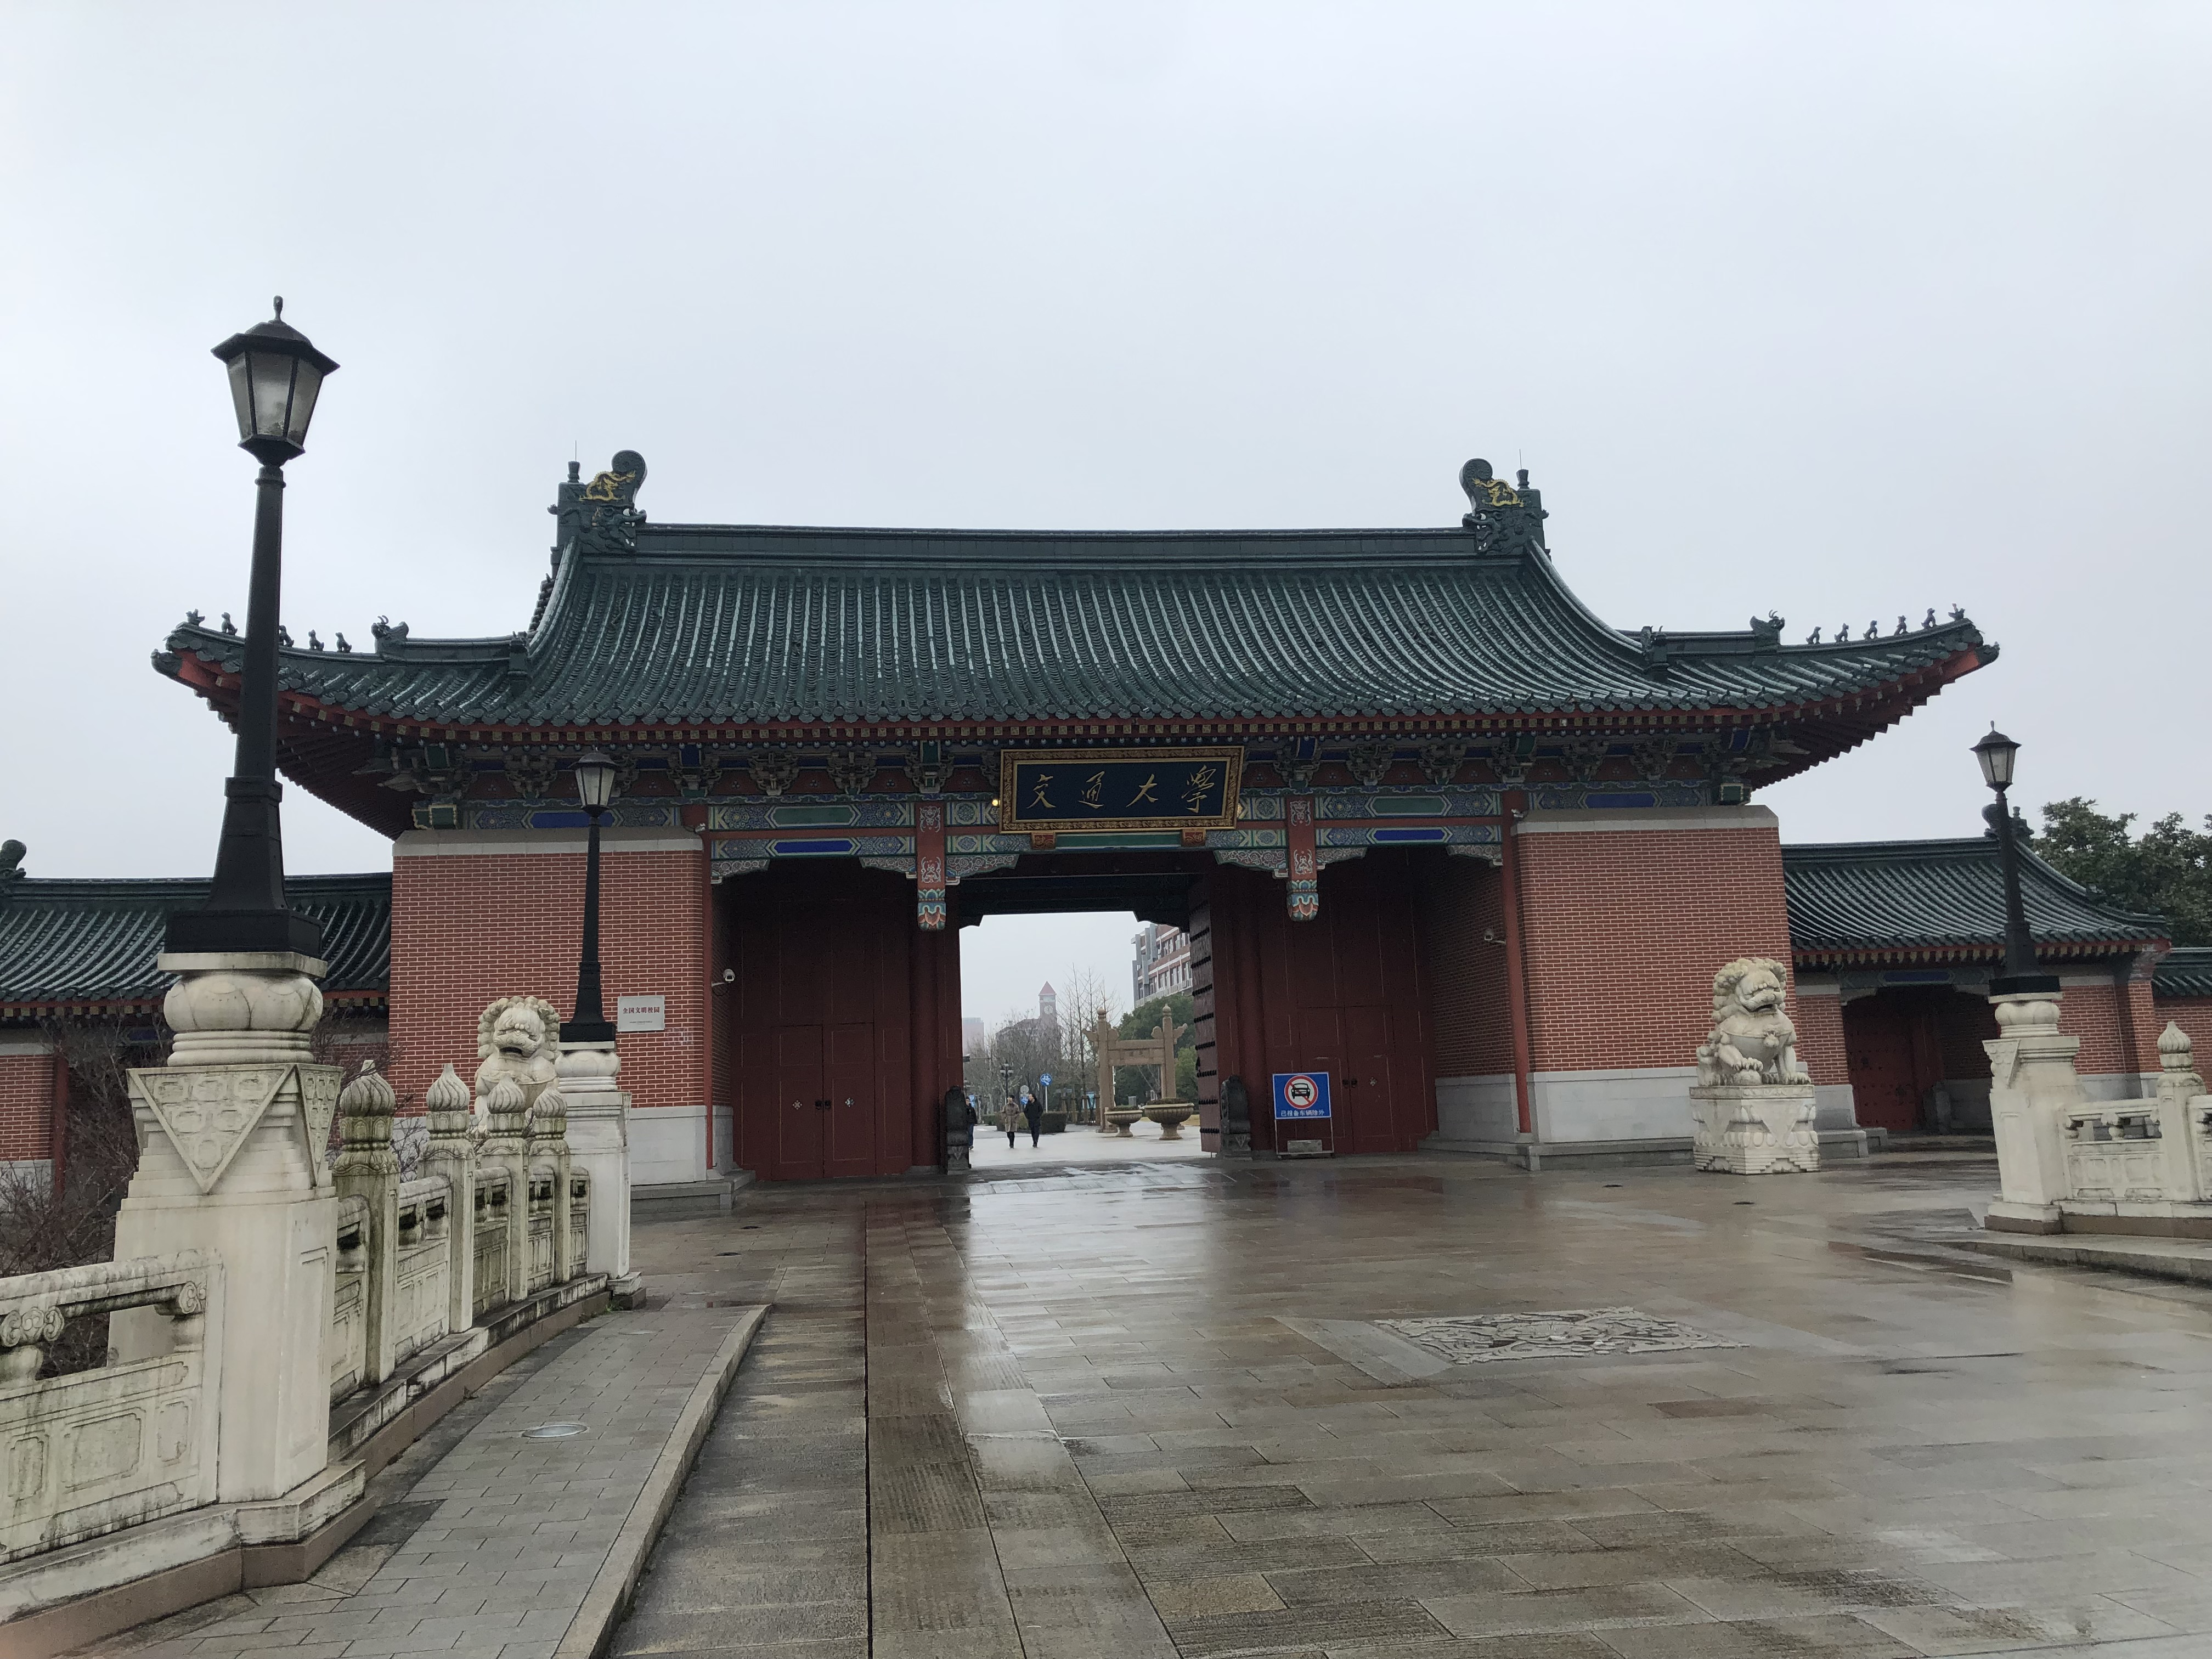
\includegraphics[width=0.3\textwidth]{/mnt/ff3bee5c-da50-4d90-848f-2a69bb4db3c8/HomeWork/SLAM_Project/1.JPG}
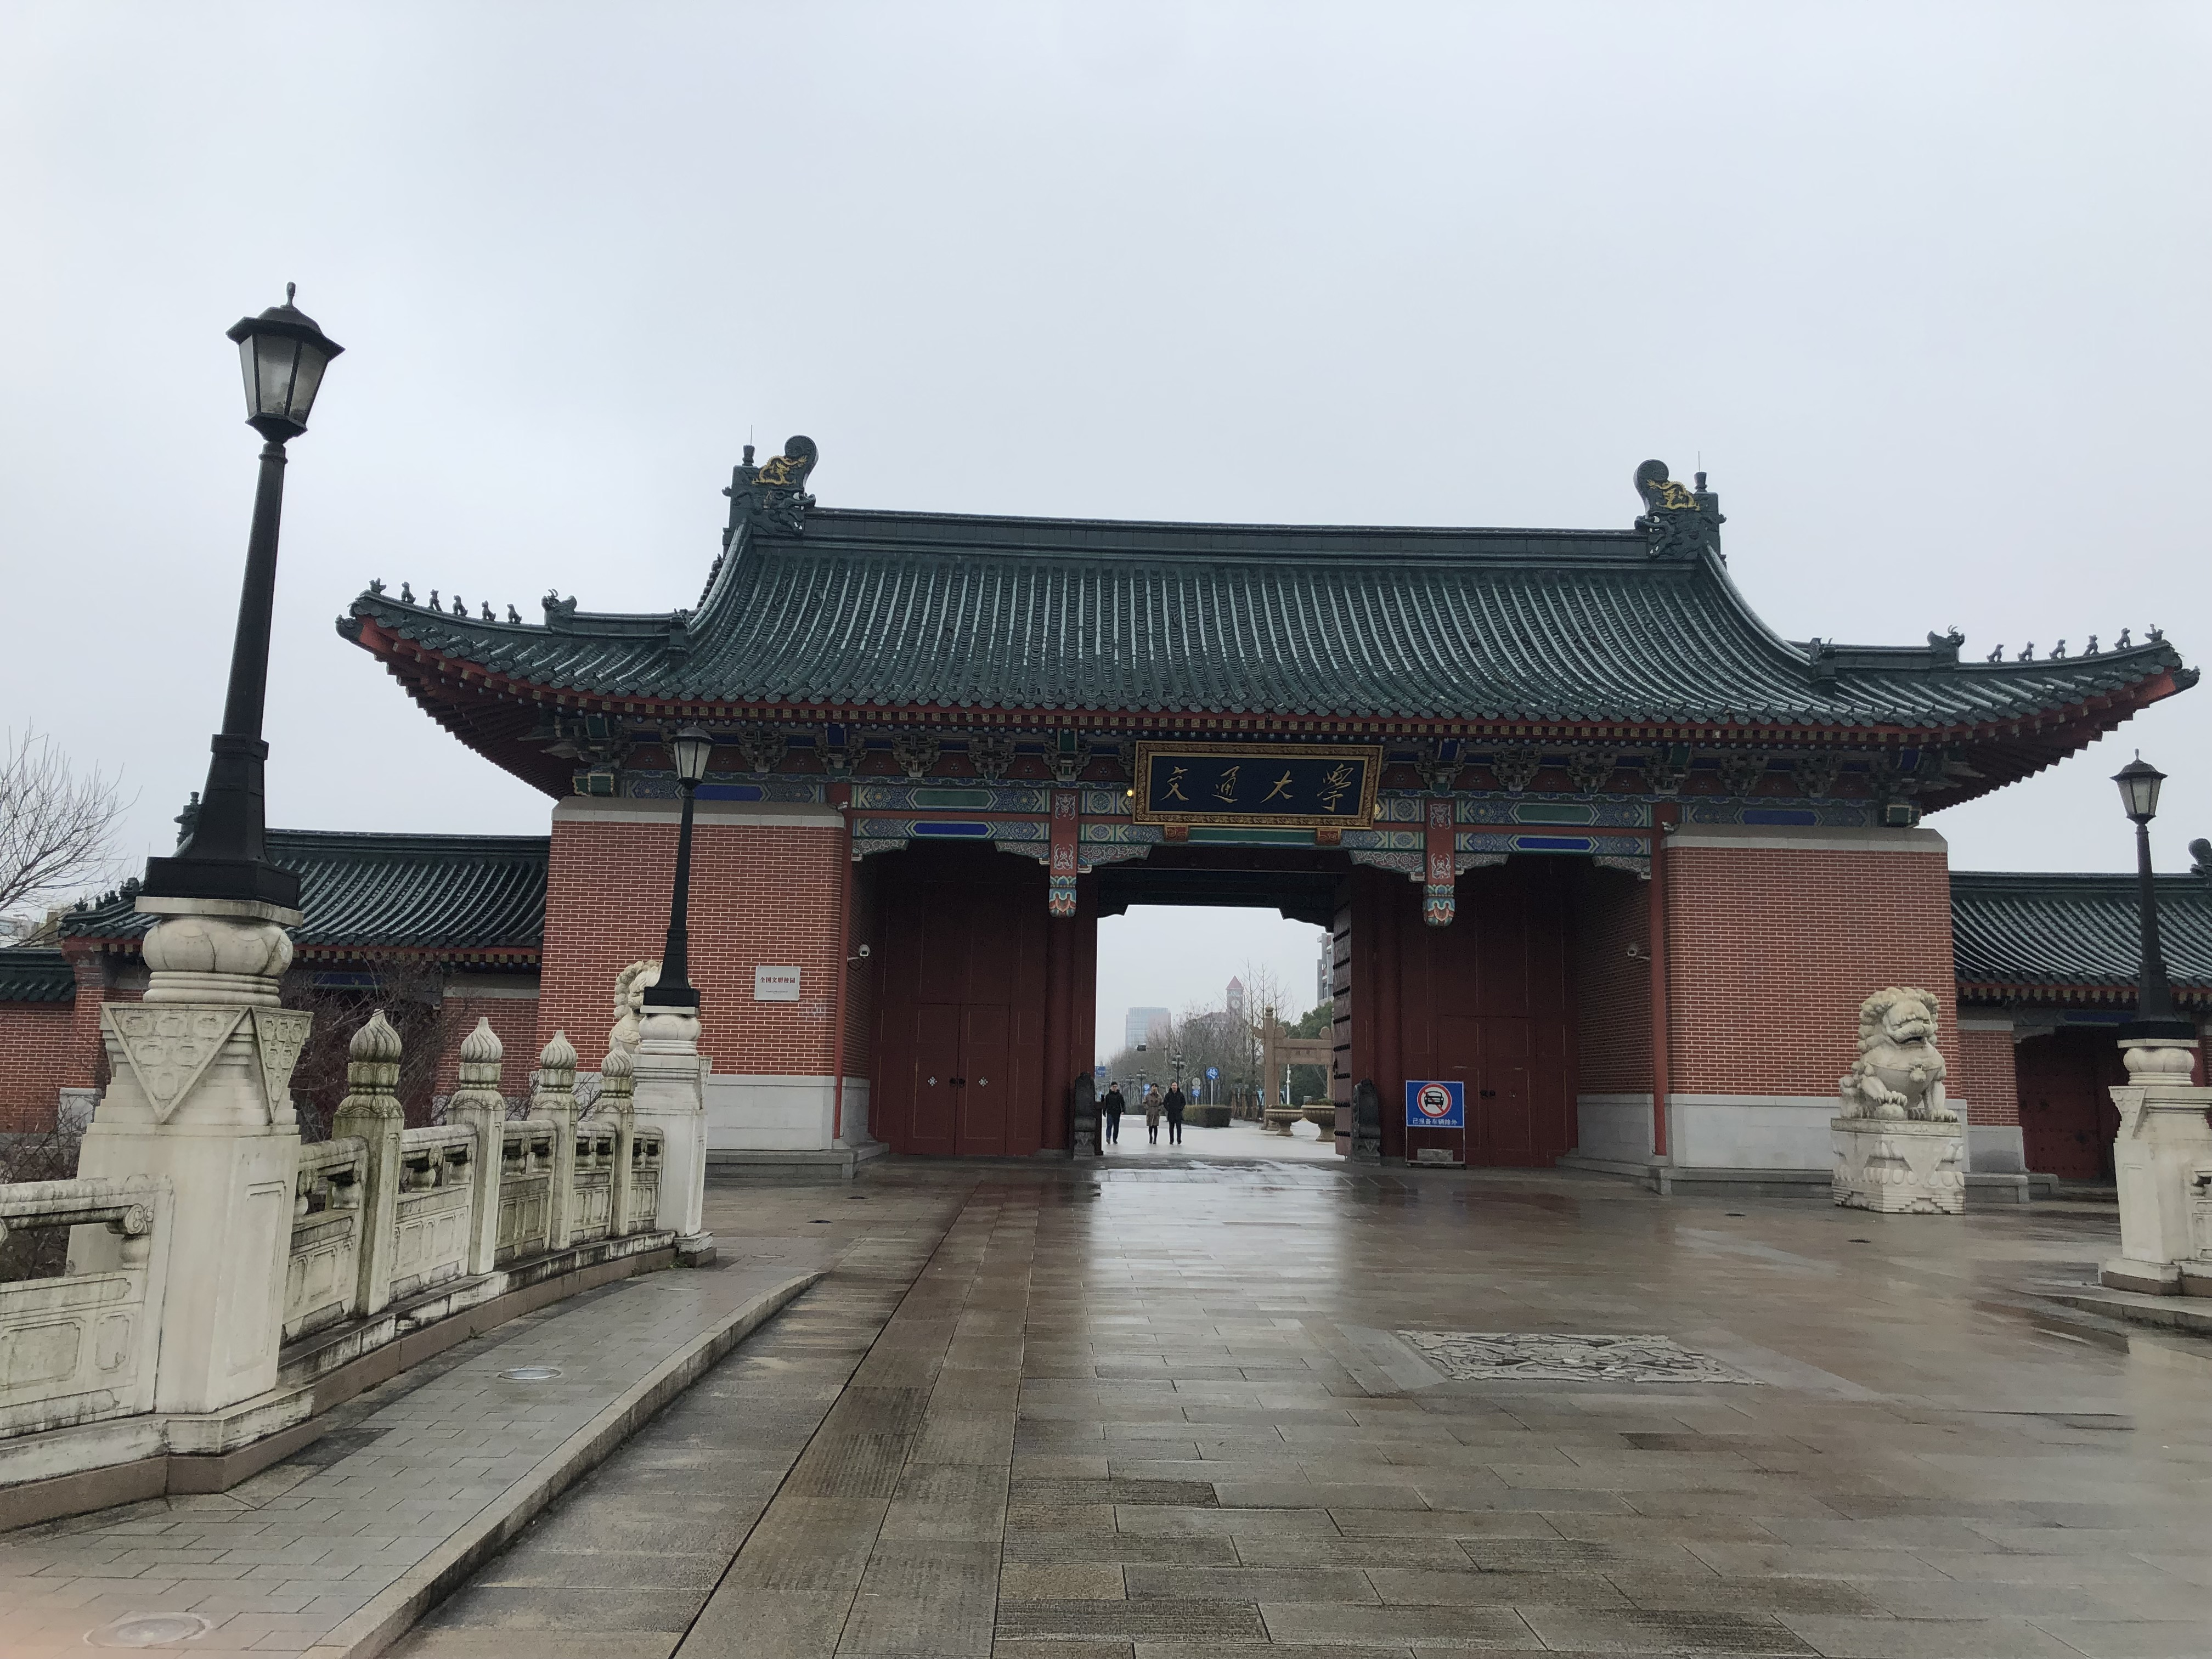
\includegraphics[width=0.3\textwidth]{/mnt/ff3bee5c-da50-4d90-848f-2a69bb4db3c8/HomeWork/SLAM_Project/2.JPG}
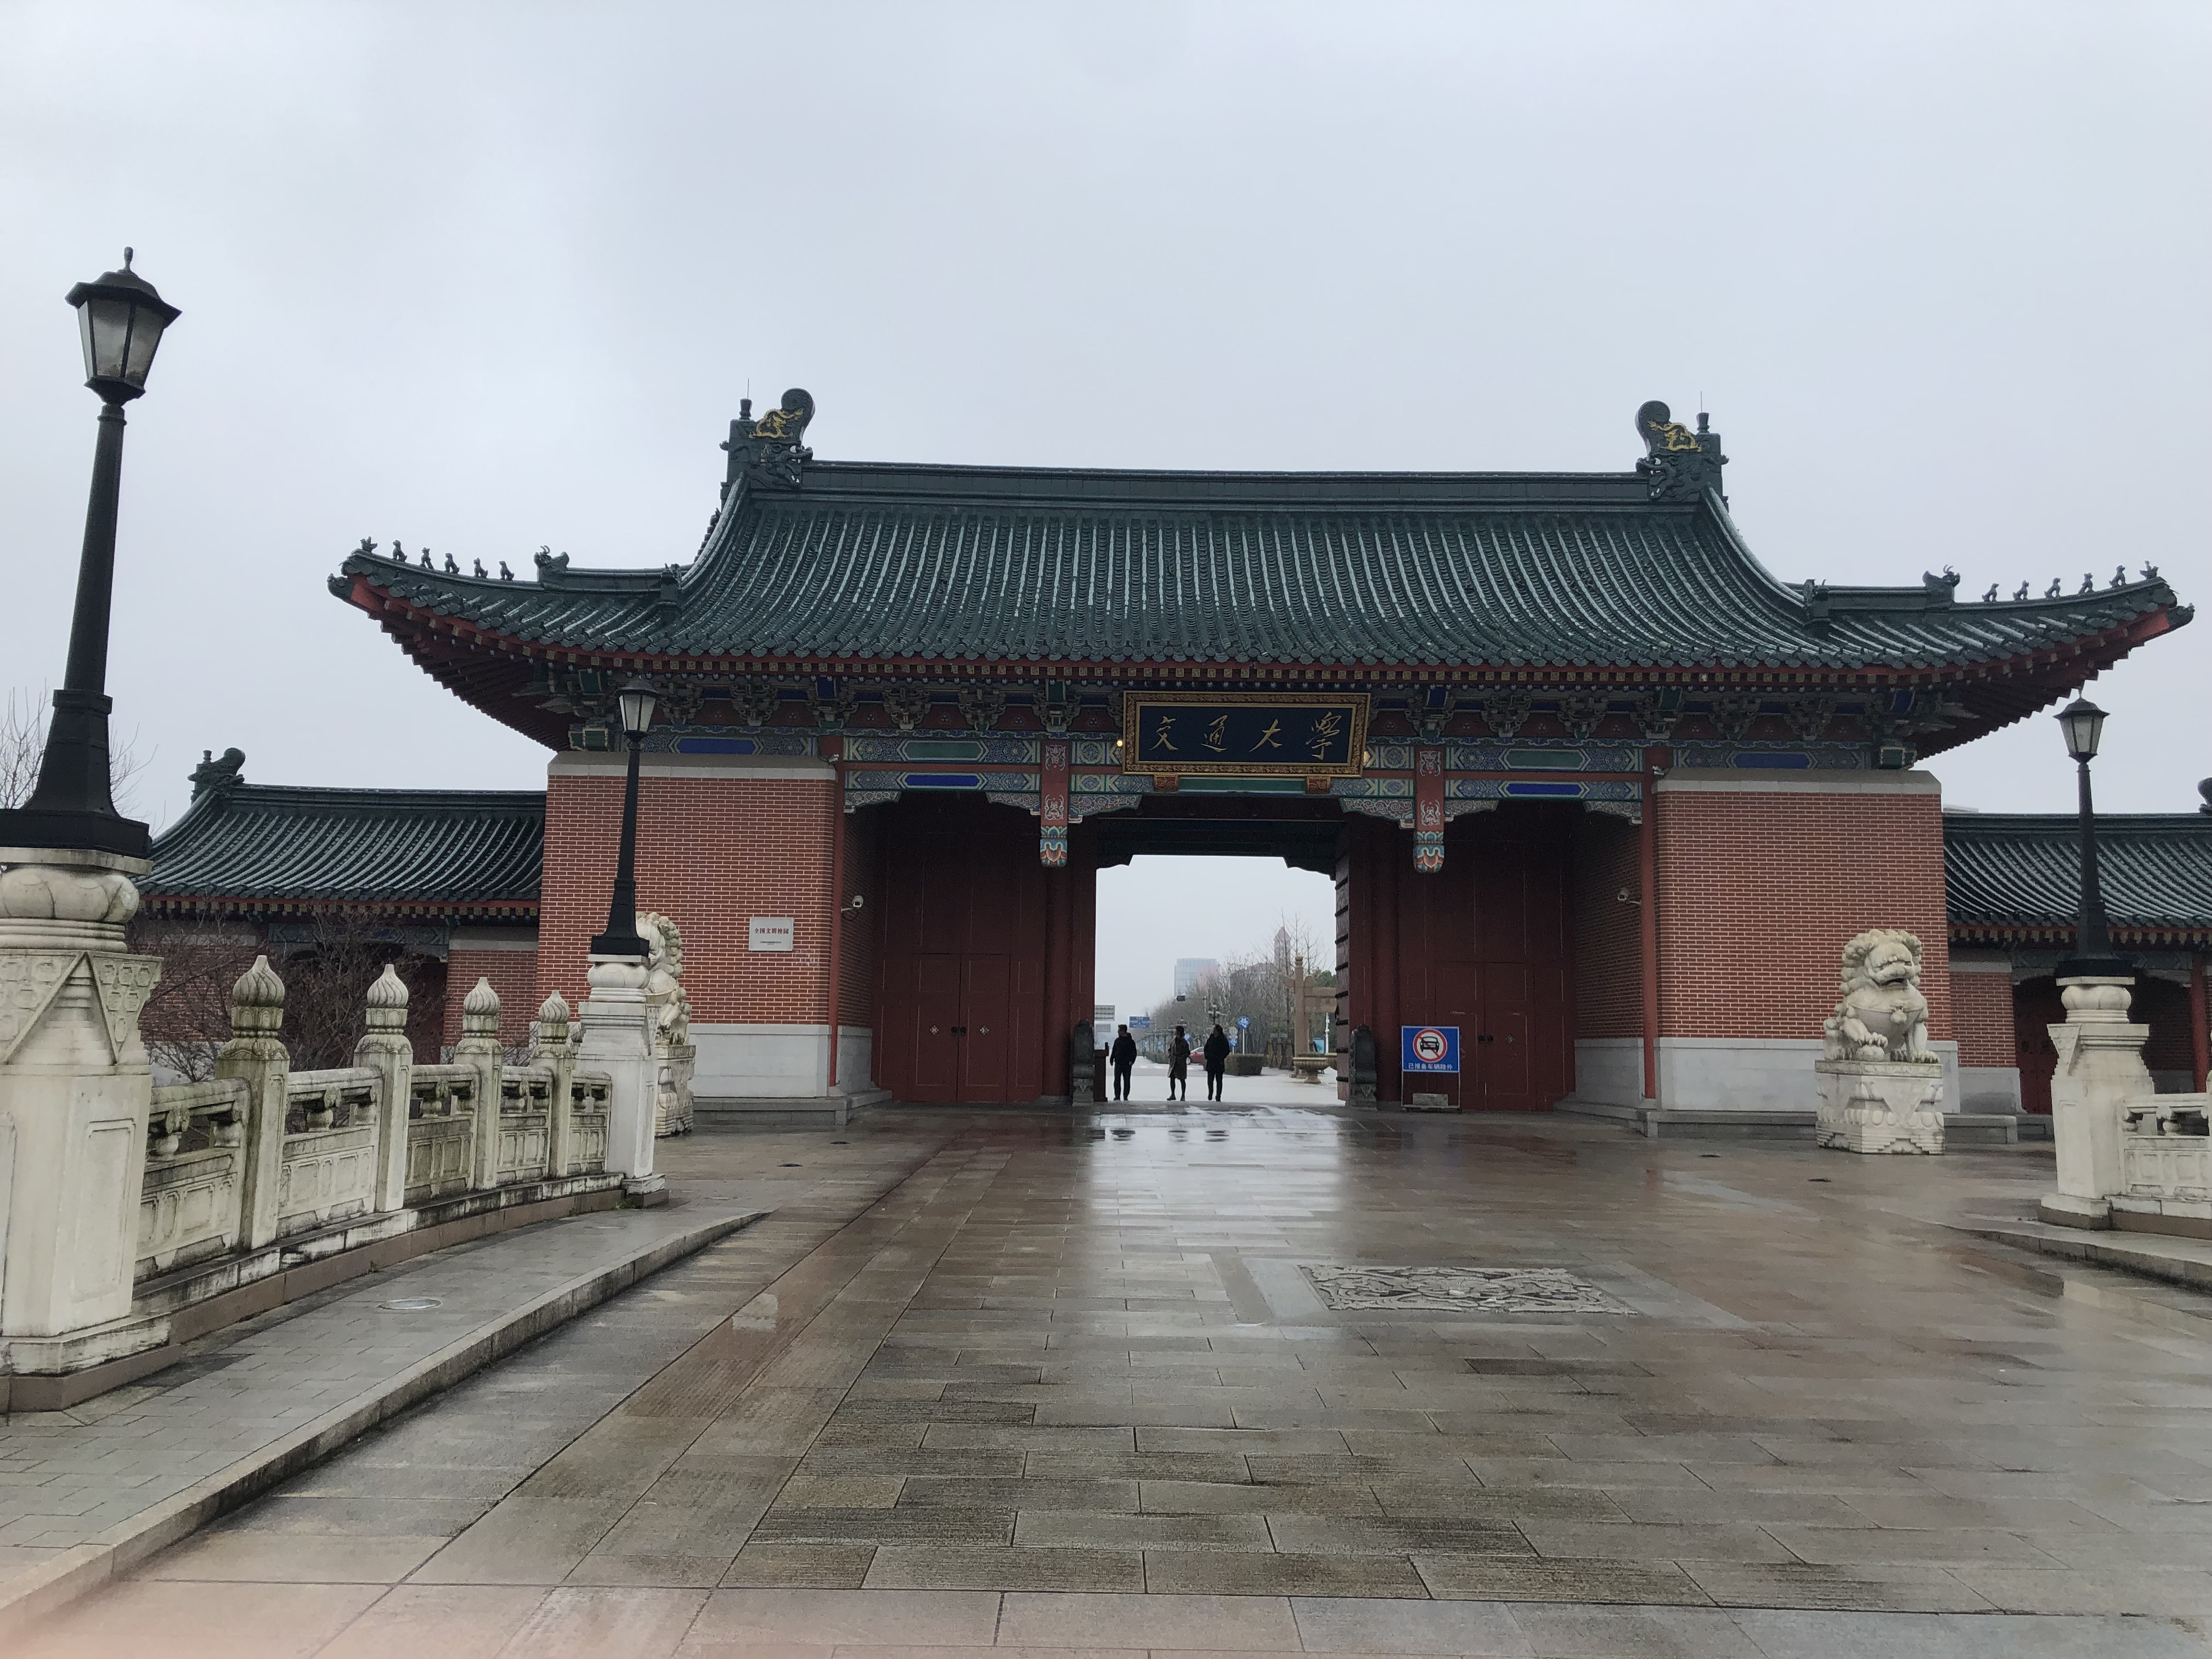
\includegraphics[width=0.3\textwidth]{/mnt/ff3bee5c-da50-4d90-848f-2a69bb4db3c8/HomeWork/SLAM_Project/3.JPG}

注:在拍摄时,所选择的场景纹理丰富,并且三维结构突出;三个拍摄角度间既要有足够的基线,也要控制相互夹角不大于30度,不然会造成后续特征点匹配的困难。

实验过程为利用拍摄的三张图片估计三次拍照的相对位姿。在实验过程中以第一次拍照的位置为轴,用相对旋转矩阵与平移矩阵来表示另外两次拍照的位姿。

